\documentclass{beamer}
\usetheme{ConnectivityLab}
\usepackage{times}
\usepackage{graphicx}
\usepackage{verbatim}
\usepackage{outlines}
\usepackage{fancyhdr}
\usepackage{subfigure}
\usepackage{cancel}
\usepackage{bibentry}
\usepackage{varwidth}
\usepackage{etoolbox}
\usepackage{epstopdf}

%%%%%%%%%%%%%%%%%%%%%%%%%%%%%%%%%%%%%%%%%%%%%%%%%%%%%%
%%%%%%%%%%%%%%%%%%%%%%%%%%%%%%%%%%%%%%%%%%%%%%%%%%%%%%

\title {
    Result of getting user info on PTT
}
\author {
    Speaker: Yin-Hong, Hsu
}
\date {
    Sep. 07, 2016 %\today
}

%%%%%%%%%%%%%%%%%%%%%%%%%%%%%%%%%%%%%%%%%%%%%%%%%%%%%%
%%%%%%%%%%%%%%%%%%%%%%%%%%%%%%%%%%%%%%%%%%%%%%%%%%%%%%

\begin{document}
\begin{frame}
    \titlepage
\end{frame}

\begin{frame}{Outline}
    \tableofcontentsgather
    \tableofcontents
\end{frame}

\section{Past}
\begin{frame}{Past}
\begin{figure}[t]
    \centering
    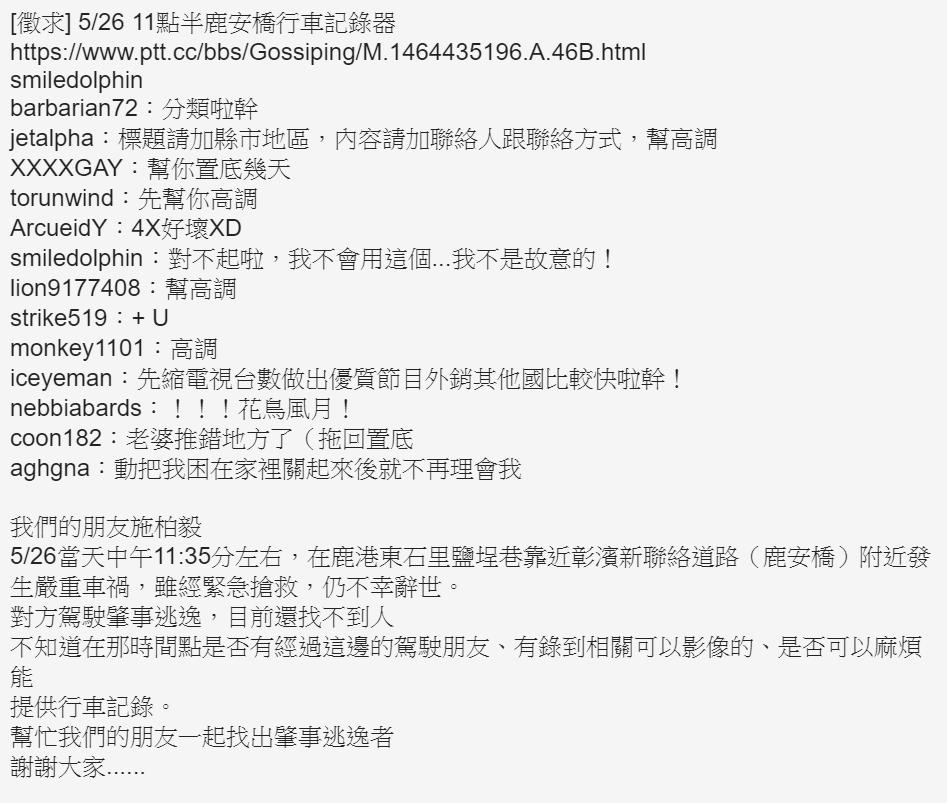
\includegraphics[width=0.7\textwidth]{figures/format.png}
    \setbeamerfont{caption}{size=\tiny}
    \caption{get post data by http}
\end{figure}
\end{frame}

\begin{frame}{Past}
\begin{figure}[t]
    \centering
    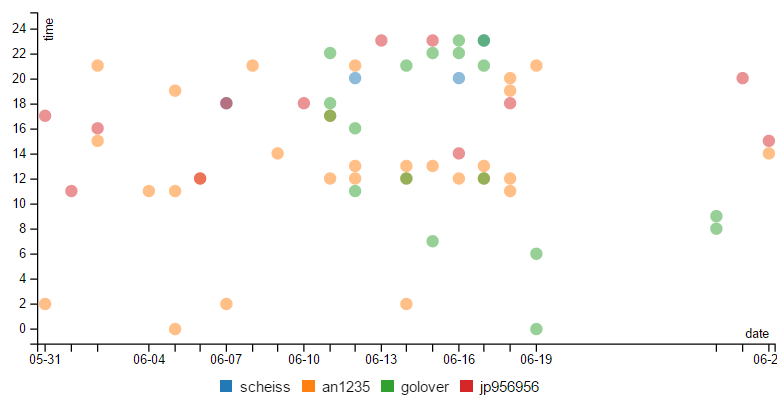
\includegraphics[width=0.9\textwidth]{figures/time.png}
    \setbeamerfont{caption}{size=\tiny}
    \caption{ analyze poster's activity }
\end{figure}
\end{frame}

\begin{frame} {Past}
\begin{figure}[t]
    \centering
    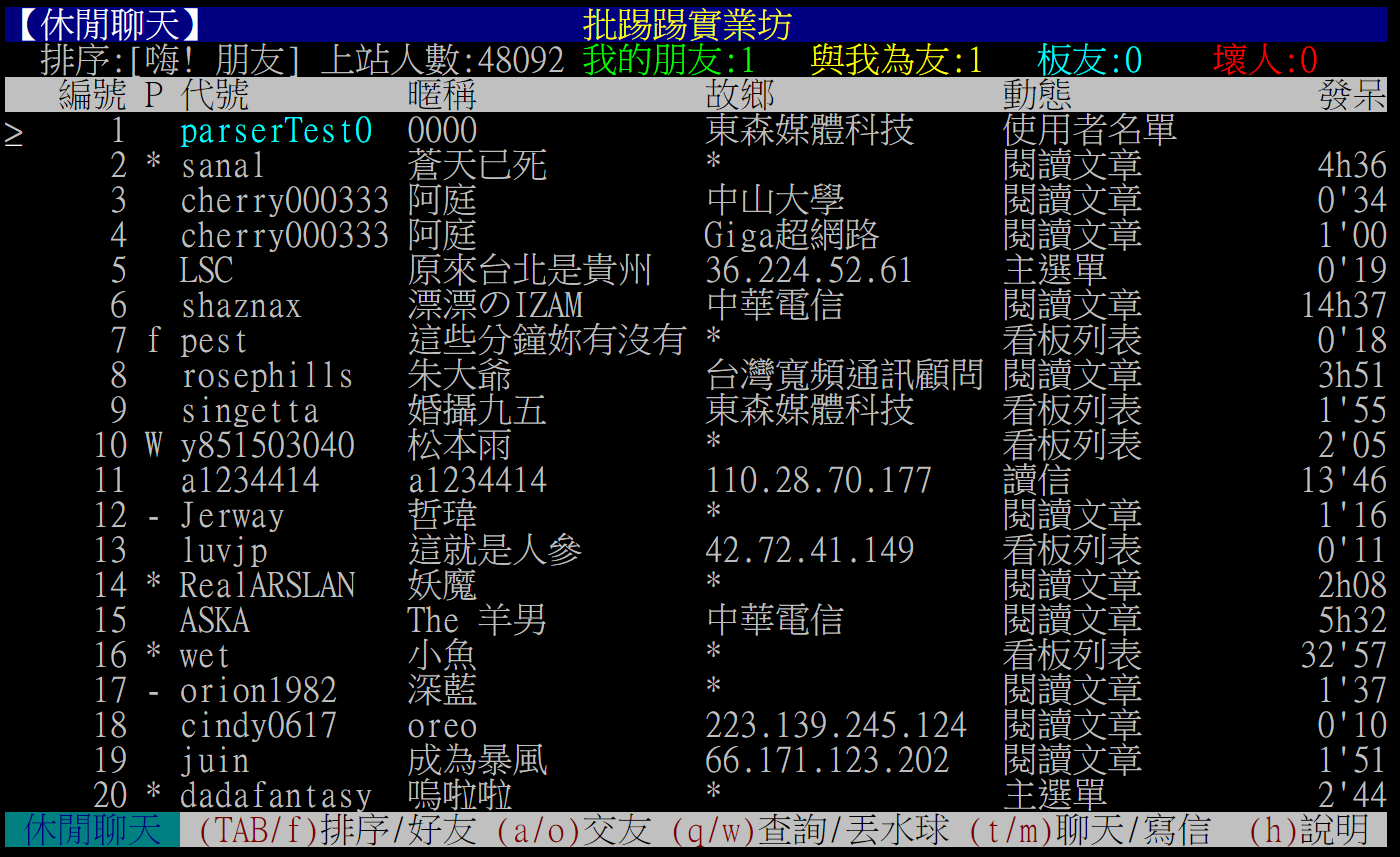
\includegraphics[width=0.9\textwidth]{figures/s3.png}
    \setbeamerfont{caption}{size=\tiny}
    \caption{Users}
\end{figure}
\end{frame}

\begin{frame} {Past}
\begin{figure}[t]
    \centering
    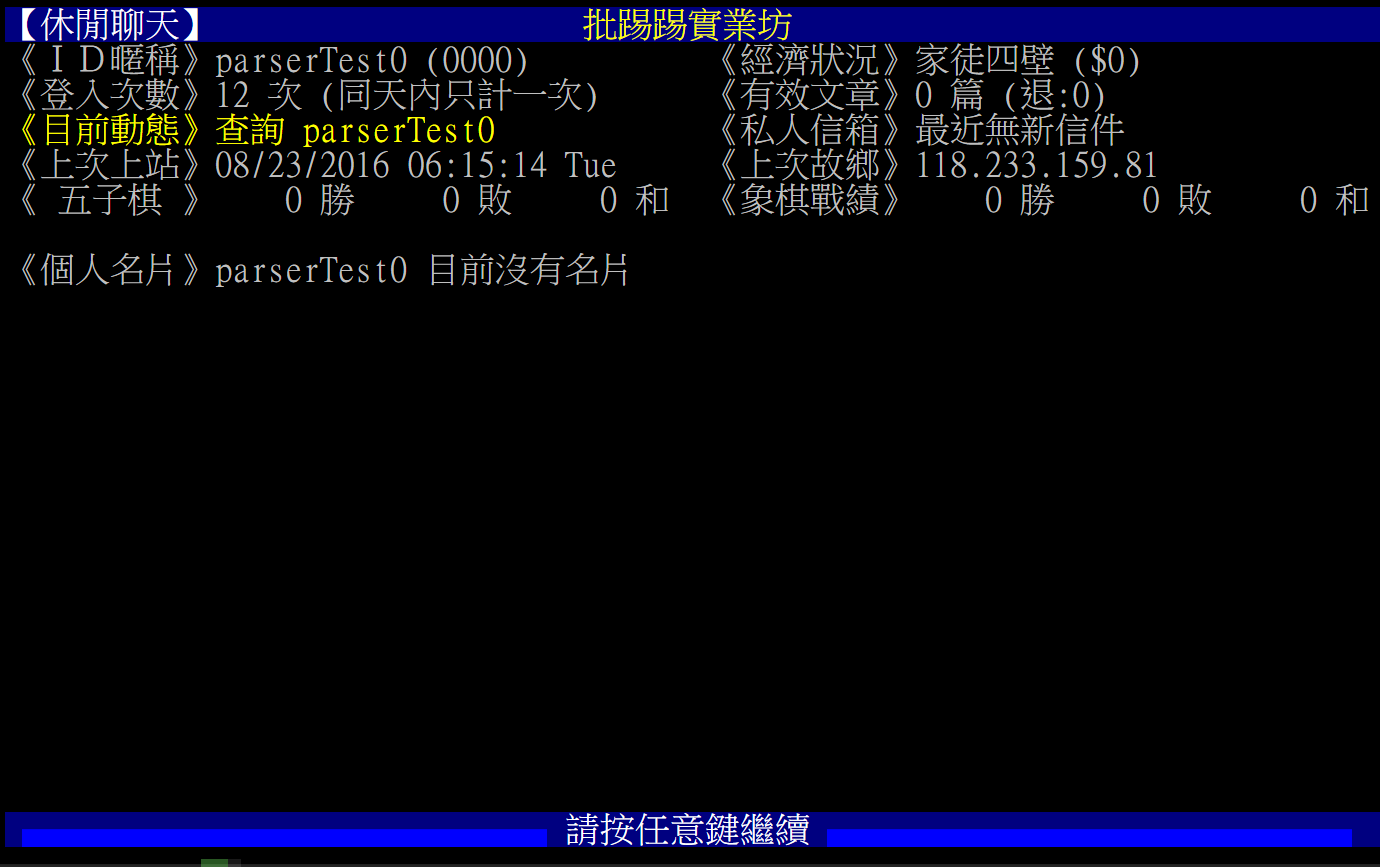
\includegraphics[width=0.9\textwidth]{figures/s4.png}
    \setbeamerfont{caption}{size=\tiny}
    \caption{Info}
\end{figure}
\end{frame}

\section{What I've done}
\begin{frame}{What I've done}
    \begin{itemize}
        \item {Parse user info from userinfo page by telnet}
        \item {Parsing User Info by telnet}
        \item {Record all data into database}
    \end{itemize}
\end{frame}

\section{The Flow Of Getting User Info}

\begin{frame} {Process}
    \begin{itemize}
        \item \textbf{UI}
        \item \textbf{No data}
        \item \textbf{Data} 
    \end{itemize}
\end{frame}

%%%%%%%%%%%%%%%%%%%%%%%%%%%%%%%%%%%%%%%%%%%%%%%%%%%%%%
%%%%%%%%%%%%%%%%%%%%%%%%%%%%%%%%%%%%%%%%%%%%%%%%%%%%%%

\begin{frame} {New}
\begin{figure}[t]
    \centering
    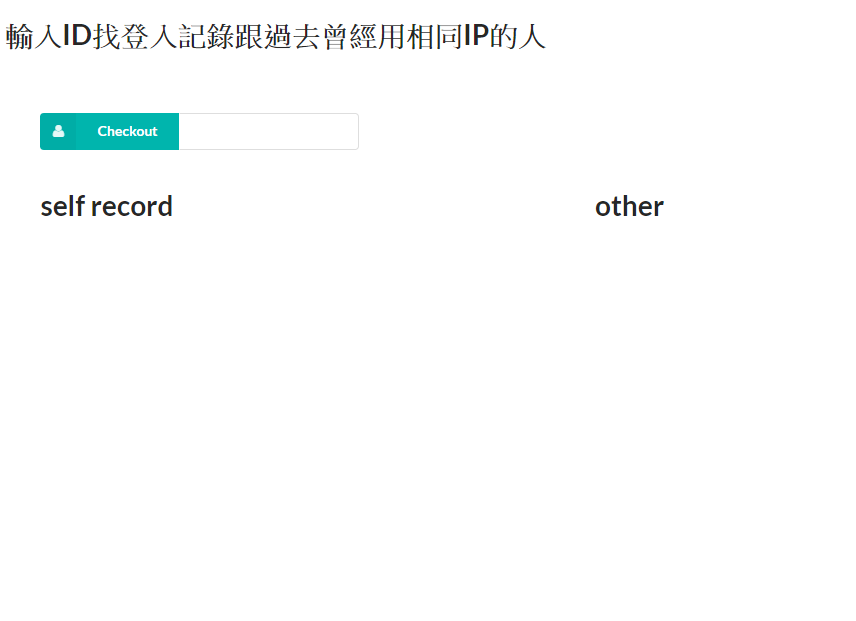
\includegraphics[width=0.9\textwidth]{figures/w1.png}
    \setbeamerfont{caption}{size=\tiny}
    \caption{UI}
\end{figure}
\end{frame}

\begin{frame} {New}
\begin{figure}[t]
    \centering
    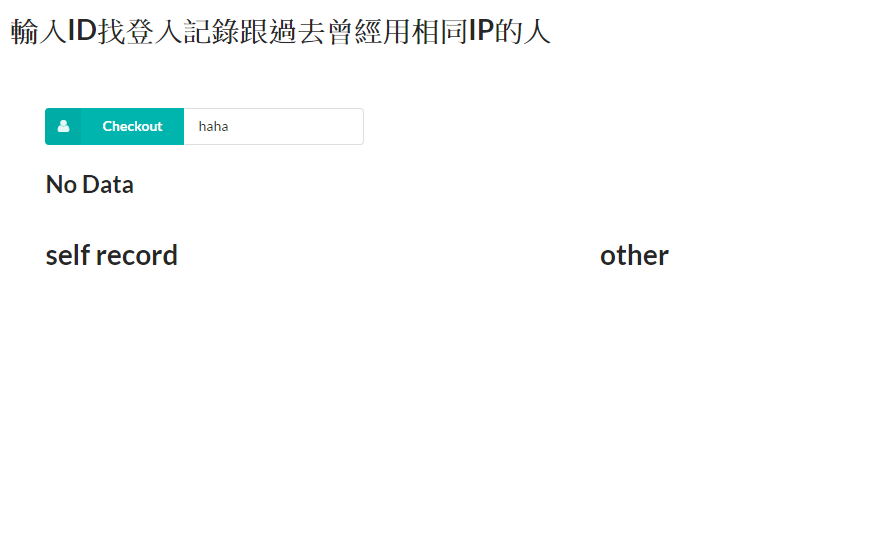
\includegraphics[width=0.9\textwidth]{figures/w3.png}
    \setbeamerfont{caption}{size=\tiny}
    \caption{No data}
\end{figure}
\end{frame}

\begin{frame} {New}
\begin{figure}[t]
    \centering
    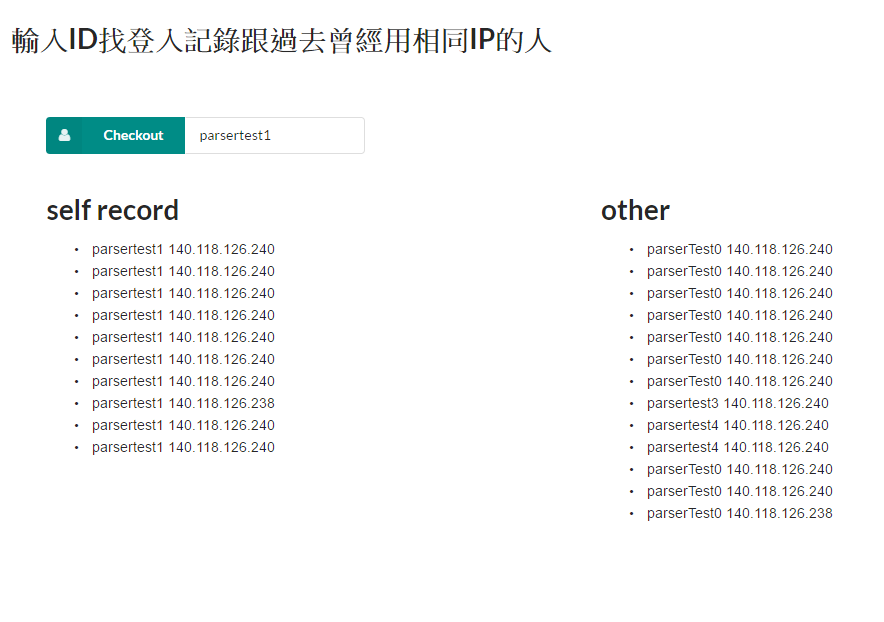
\includegraphics[width=0.9\textwidth]{figures/w2.png}
    \setbeamerfont{caption}{size=\tiny}
    \caption{Data}
\end{figure}
\end{frame}

%%%%%%%%%%%%%%%%%%%%%%%%%%%%%%%%%%%%%%%%%%%%%%%%%%%%%%
%%%%%%%%%%%%%%%%%%%%%%%%%%%%%%%%%%%%%%%%%%%%%%%%%%%%%%


\section{}

\end{document}
